
\section{Projektvorschlag vom 22.09.2025}\label{sec:projektvorschlag}

\section*{Schwerpunkt Rendering: Geometry Wars Klon}

\subsection{Anforderungen}

In der Projektarbeit wird ein Klon zu dem Spiel Geometry Wars\footnote{
\url{https://en.wikipedia.org/wiki/Geometry_Wars}
} erstellt, ein Top-Down Twin-Stick Shooter.\\

\noindent
Insgesamt dauert ein Spieldurchlauf 3 Minuten, oder bis der Spieler alle Schiffe verloren hat. Ziel ist es, die immer größer werdenden Gegnerwellen zu überdauern und dabei möglichst viel Punkte zu sammeln.



\subsection{Spielfunktionen}
\begin{itemize}
    \itemsep0.5em
    \item \textbf{Einzelspieler}
    \begin{itemize}
        \item Es gibt einen Spielmodus, den \textbf{Time-Attack-Modus}: Das Spiel gilt als erfolgreich beendet, wenn der Spieler eine Zeit von 3 Minuten überdauert.
    \end{itemize}
\end{itemize}

\subsection{Architektur}

Die Spieleengine ist nach \textit{first principles} aufgebaut und besitzt im Groben drei architektonische Schichten (s. Abbildung~\ref{fig:architecture}), die selbstständig erarbeitet werden:

\begin{enumerate}
    \item Applikationsschicht, die die Initialisierung und Verwaltung eines Event-Systems, Input Managers, Audio Managers und des Fenster Systems übernimmt. Notwendige SDKs, die diese Funktionen bereitstellen\footnote{
        sofern die Zeit es erlaubt, bspw. Audio wie \textbf{fmod} (\url{https://www.fmod.com})
    } sowie Fenstermanagement und Input (bspw. \textbf{glfw}\footnote{\url{https://www.glfw.org/}}), werden als vendor code von dem Spiel genutzt und über eine API gekapselt, damit die Applikationsschicht agnostisch hinsichtlich der verwendeten Libs ist (Adapter bzw. Wrapper).
    \item Render Engine: Als Rendering Backend wird OpenGL benutzt. Benötigte Schnittstellen werden über GL-loader wie \textbf{glad}\footnote{
        \url{https://glad.dav1d.de/}
    } bereitgestellt.
    \item Game Engine: Die Game Engine wird auf die Umsetzung des Geometry Wars hin ausgerichtet. Dies soll vor allem weitere notwendige Abstraktionsschichten wie eine flexible und anpassbare Physikengine unnötig machen.
\end{enumerate}

\begin{figure}
    \centering
    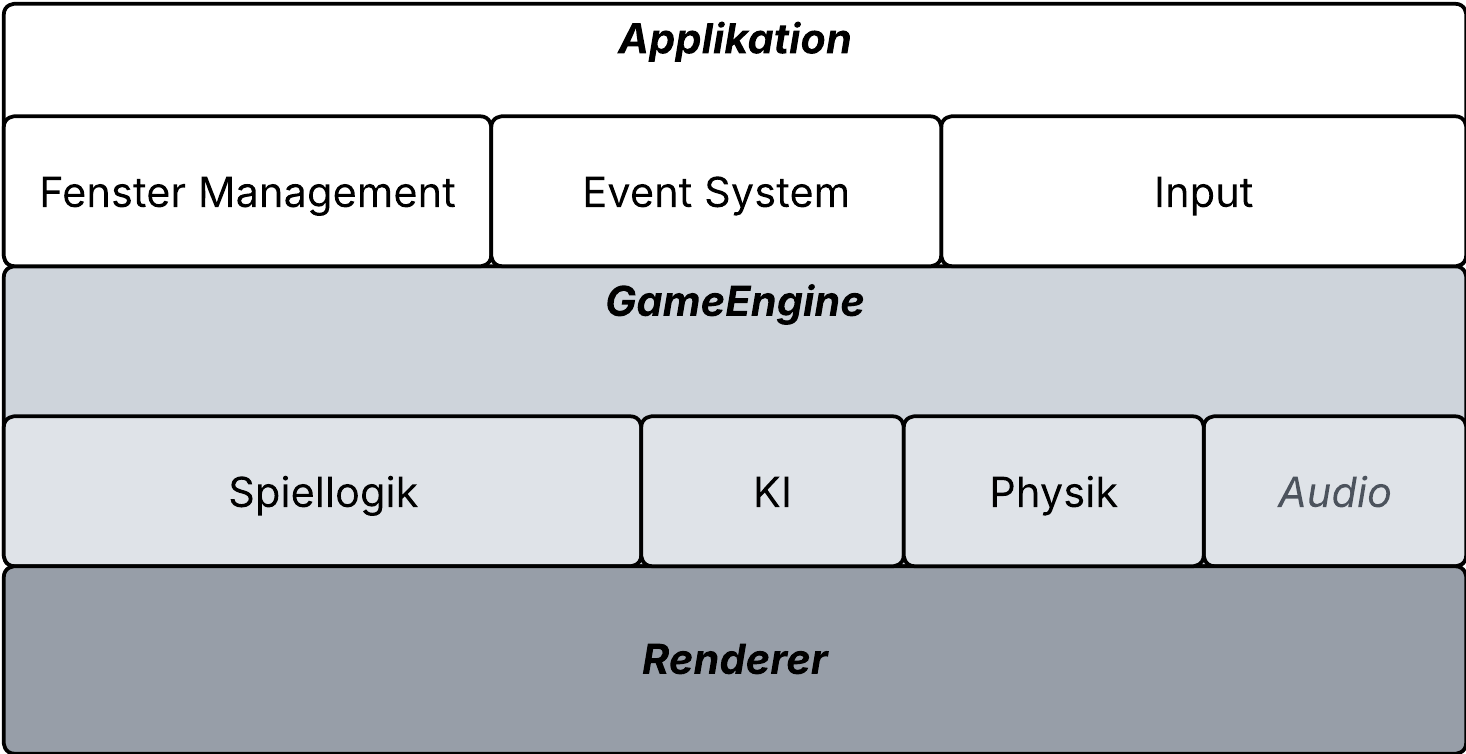
\includegraphics[width=1\columnwidth]{appendix/img/architecture}
    \caption{Vereinfachte Darstellung der Schichtenarchitektur des umzusetzenden Spiels. Das Audio-System ist hierbei berücksichtigt, auch wenn es bzgl. des Scopes keine Priorität hat.}
    \label{fig:architecture}
\end{figure}

\\


Die Physikengine soll auf die Anforderungen eines 2D-Shooters hin ausgerichtet sein (Bewegungsphysik basierend auf einfachen Vektoren in einer Ebene), die Kollisionsabfrage soll zuverlässig und performant funktionieren.


\subsection{Zielsetzung}

Diese Projektarbeit setzt den Fokus auf eine saubere Architektur sowie eine nachvollziehbare Umsetzung in der Programmiersprache C++$\ge$20.\\
Für die Darstellung des Spiels wird auf geometrische Primitive zurückgegriffen, so dass am Schluss ein Spiel entsteht das komplett auf Sprites verzichtet und die Darstellung aller benötigten Spielinformationen über Polygone und Linien realisiert (Fonts ausgenommen).

\noindent
Ein (messbarer) Schwerpunkt des Spiels ist eine stabile Framerate von $\ge$ 60 FPS bei einer Auflösung von $1920 \times 1080$.
Für die Entwicklung steht eine Grafikkarte vom Typ \textit{Nvidia GeForce RTX 5090} zur Verfügung, getestet werden kann außerdem auf einem Laptop mit einer \textit{Nvidia GTX 1070} Grafikkarte.
Die Lastparameter können also durchaus noch angepasst werden.\\
Die Herausforderung besteht hier in der anzuwendenden Technik bei der Darstellung von mehreren Hundert Gegnerobjekten auf dem Screen zur selben Zeit (\textit{Instancing}), Kollisionsabfrage mit dem Spieleschiff sowie den abgefeuerten Waffen und dem Gegnerverhalten bei entsprechender Steuerung des Spielerschiffes.\\
Ein nicht unwesentlicher Punkt bei der Umsetzung des Spiels ist der \textit{Game Feel}(\cite{Swi09})\footnote{
auch: \textit{Game Juice}
}: Das Spielererlebnis soll durch visuelles Trefferfeedback durch Partikeleffekte unterstützt werden.\\

\noindent
Die Gegner-KI basiert auf einem einfachen \textit{Spawn and Seek}-Verhalten mit einer zusätzlichen Drift-Komponente, die je nach Gegnertyp variiert. Für die Umsetzung sind 2-3 grundlegende Gegnertypen geplant:
\begin{itemize}
\itemsep0.5em
\item \textbf{Schneller Typ:} Geringe Widerstandsfähigkeit (wenig Schilde).
\item \textbf{Langsamer Typ:} Hohe Widerstandsfähigkeit (viele Schilde).
\item \textbf{Schwarm-Typ:} Mittlere Geschwindigkeit, keine Schilde, tritt in großer Anzahl als exklusive Gegnerwelle auf.
\end{itemize}

\noindent
Zur Steuerung des Spiels wird ein Gamecontroller wie der Xbox Elite Controller\footnote{
\url{https://www.xbox.com/de-DE/accessories/xbox-elite-controllers}
} bzw. der PS5 DualSense Wireless Controller\footnote{
\url{https://www.playstation.com/de-de/accessories/dualsense-wireless-controller/}
} vorausgesetzt.

\subsection{Vorgeschlagener Zeitplan}

\begin{itemize}
\itemsep0.5em
\item 20.10.2025: Bereitstellung der Applikationsschicht inkl. Implementierung des Event Systems, Input Managers sowie Anbindung an das Low Level API-Sub-Systems
\item 17.11.2025: Bereitstellung der Rendering Engine. Erster Entwurf des Spielfeldes samt Darstellung des Spielerschiffs.
\item 22.12.2025: Umsetzung der Physik und Spielereingabe zur Steuerung des Schiffs, Feuermechaniken
\item 19.01.2026: Implementierung der wichtigsten Spielregeln - und Mechaniken. Spielfähiger Prototyp.
\item 09.02.2026: Bereitstellung des umgesetzten Prototyps. Feinschliff.
\item 16.03.2026: Abgabe der Dokumentation und Vorstellung des Projekts.
\end{itemize}
